
\chapter{Getting Started}

CFAST is documented by three publications, this user's guide, a technical reference guide~\cite{CFAST_Tech_Guide_7} and a model evaluation guide \cite{CFAST_Valid_Guide_7}. The technical reference guide describes the underlying physical principles, provides a comparison with other models, and includes an evaluation of the model following the guidelines of ASTM~E1355~\cite{ASTM:E1355}. The model evaluation guide documents verification and validation efforts for the model. This user's guide describes how to use the model.

\section{Installation}

CFAST was designed primarily for a personal computer running Microsoft Windows. However, the source code is written in Fortran and can be run as a stand alone command line application that reads input data from a text file. Details of how one runs CFAST without the Windows-based graphical user interface are found in Appendix~\ref{sec:CFAST_Keywords}. All of the files associated with CFAST can be obtained at:
\begin{lstlisting}
http://cfast.nist.gov
\end{lstlisting}
The CFAST distribution consists of a self-extracting set-up program for Windows-based personal computers. After downloading the set-up program, double-clicking on the file's icon walks you through a series of steps for installation of the program.  The most important part of the installation is the creation of a folder ({\ct C:$\backslash$Program Files$\backslash$CFAST} by default) in which the CFAST executable files and supplemental data files are installed.  Sample input files are found in the {\ct Examples} folder.

CFAST input files are best created and run using a Windows-based input editor called CEdit. Sample input files are provided with the program for new users who are encouraged to first run the sample calculations before attempting to create an input file. To run the model, browse to the location of the CFAST sample input file (default location is in a folder called {\ct Examples} in the installation folder, copy the file named {\ct standard.in} to a location of your choice and then double click on the copied file. This should open the file in the CFAST input editor, CEdit, as shown in Fig.~\ref{primary_screen}.
\begin{figure}[h!]
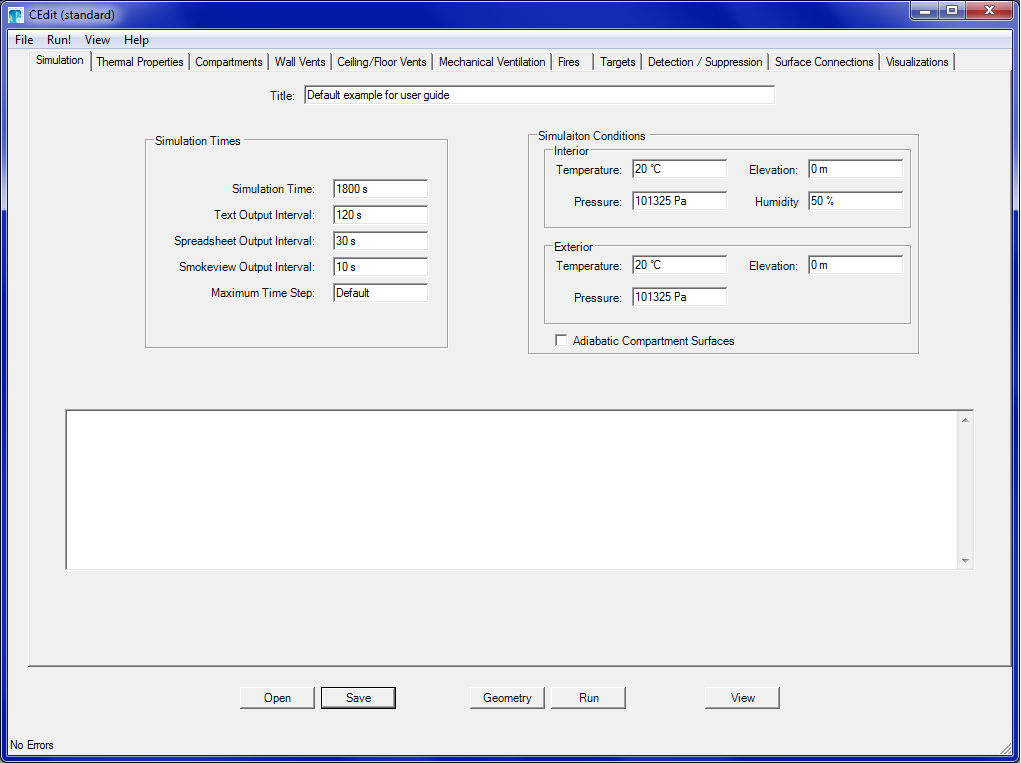
\includegraphics[width=6.5in]{FIGURES/Running_CFAST/Environment_Tab}
\caption[The Primary CFAST Input Page]{The Primary CFAST Input Page.}
\label{primary_screen}
\end{figure}
The simple test case can be run from the program menu by clicking on the ``Run'' icon. The case should finish in a few seconds. To verify that the installation has been done correctly, the output of the model should appear as shown in Fig.~\ref{Run_Model}.
\begin{figure}[h!]
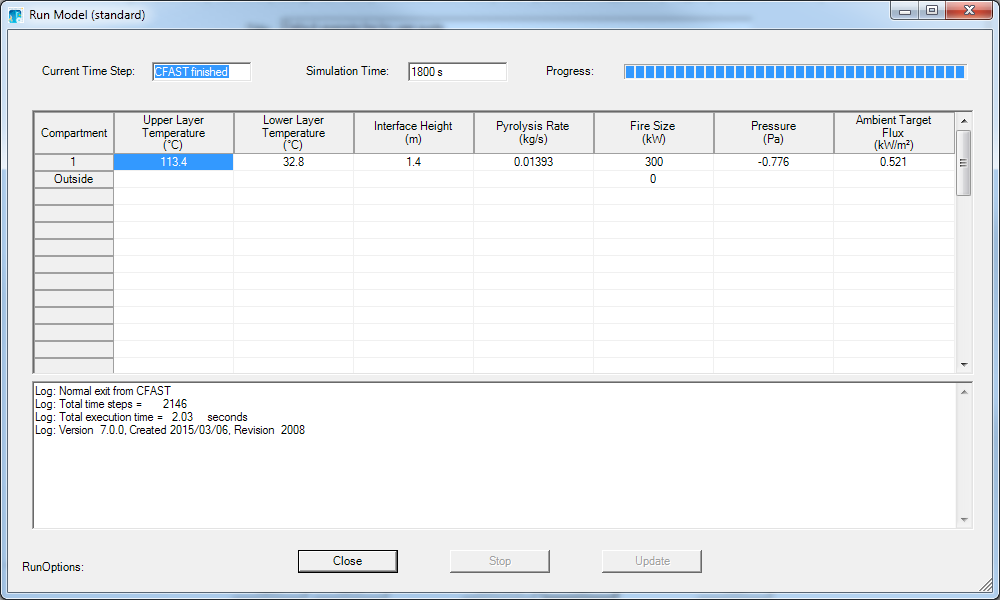
\includegraphics[width=6.5in]{FIGURES/Getting_Started/Standard_Output}
\caption[The Standard CFAST Output Screen]{The Standard CFAST Output Screen.}
\label{Run_Model}
\end{figure}


\section{Basic Features}

The input parameters are organized via tabs near the top of the CEdit screen, as shown in Fig.~\ref{primary_screen}.
\begin{description}
\item[Simulation Environment] includes simulation time, specification of model outputs, and ambient conditions. Also included on the page are a constantly updated list of errors, warnings, and messages about the input file specification or model simulation.
\item[Thermal Properties] defines the thermal conductivity, specific heat, density, thickness and emissivity values for all materials and fuel sources to be used in a simulation.
\item[Compartments] defines the size, construction characteristics, and position of the compartments in a simulation.
\item[Wall Vents] define doors and windows.
\item[Ceiling/Floor Vents] define holes in the ceiling/floor.
\item[Mechanical Ventilation] defines forced air ventilation.
\item[Fires] include user specification of the initial fire source and any additional burning objects in one or more of the compartments of the simulation.
\item[Targets] provide the ability to calculate the temperature and net heat flux to objects placed and oriented arbitrarily in the structure.
\item[Detection / Suppression] defines any heat alarms and sprinklers in the compartments of the simulation.
\item[Surface Connections] allows for more detailed description of the connections between compartments in the simulation to better simulate the transfer of heat from compartment to compartment in the simulation.
\item[Visualizations] allows specification of one or more 2-D and 3-D visualizations to be added to the simulation for viewing with Smokeview. Note that these can require significant additional computational time than a basic CFAST simulation without visualizations.
\end{description}


\section{The Run! Menu}

The program includes a number of menu items for ancillary functions.  In addition to the normal file menu items to open and save input data files or to exit the program, a `Run!' menu is included to execute or view the current simulation. Menu items include the following:
\begin{description}
\item[Create Geometry File] for visualization with the program Smokeview.  The input data file is saved, if necessary, and CFAST is run with an option to only run through initialization. This is particularly useful to review placement of compartments, vents, and fires in a CFAST scenario. The resulting geometry can be viewed with the `Simulation Visualization, Smokeview' menu item, below.
\item[Model Simulation, CFAST] runs the case. The input file is saved, if necessary, and CFAST is run to completion.
\item[Simulation Visualization, Smokeview] runs the program Smokeview with the currently defined geometry.
\item[Output Options] include:
\begin{description}
\item[Total Mass Output File] If checked, this menu item directs the CFAST model to replace the flow output with total mass flow through (mechanical) vents rather than the default flow rate values.
\item[Net Heat Flux]  If checked, this menu item directs the CFAST model to calculate heat flux to targets as a net heat flux to the target with the target at ambient temperature rather than at the calculated temperature.  This output is particularly useful to compare predictions to heat flux measurement using water cooled heat flux gauges.
\item[Show CFAST Window] If checked, this menu item allows the user to see the windows command prompt that is used to execute the CFAST model when the Model Simulation, CFAST menu item is used.  By default, this is not checked.  Normally, this can be left unchecked.  For troubleshooting, this can be selected to see additional details of the calculation as it progresses.
\item[CFAST Validation Output] If checked, this menu item directs the CFAST model to output an abbreviated heading for spreadsheet columns that are better for automated processing of the data. Heat fluxes are output as net heat flux to and ambient temperature target consistent with measurement with temperature-controlled heat fluxes gauges.
\end{description}
\end{description}


\section{The View Menu}

The View menu allows you to view or print the input data file, output file (if the simulation has been run and a text output file generated) and the log file of the simulation. If one of the items does not exist on the user's hard disk, the selection is grayed out.
\begin{description}
\item[Select Engineering Units] allows you to select the units for input and output. By default, most outputs are in S.I. units, with temperature in Celsius.
\end{description}


\section{The Help Menu}

The Help menu accesses this user's guide, the CFAST web site, or an about dialog box that displays the user license and version of the program.







